%!TEX root = ../thesis.tex

\chapter{Introduction}%
\label{chap:introduction}


This is a complete template for the MSc Geomatics thesis.
It contains all the parts that are required and is structured in such a way that most/all supervisors expect.
Observe that the MSc Geomatics at TU Delft has no formal requirements, how the document looks like (fonts, margins, headers, etc) is entirely up to you.

We basically took the template \texttt{KOMA-Script scrbook}, added the front/back matters (cover page, copyright, abstract, etc.), and gave examples for the insertion of figures, tables and algorithms.

\emph{It is not an official template and it is not mandatory to use it.}

But we hope it will encourage everyone to use \LaTeX\ for writing their thesis, and we also hope that it will \emph{discourage} some from using Word.

If you run into mistakes/problems/issues, please report them on the GitHub page, and if you fix an error, then please submit a pull request.

\url{https://github.com/tudelft3d/msc_geomatics_thesis_template}.


%%%
%
\section{How to get started with \LaTeX?}%
\label{sec:startlatex}



Follow the Overleaf's Learn LaTeX in 30min (\url{https://www.overleaf.com/learn/latex/Learn_LaTeX_in_30_minutes}) to start.

The only crucial thing missing from it is how to add references, for this we suggest you use \texttt{natbib} tutorial (\url{https://www.overleaf.com/learn/latex/Bibliography_management_with_natbib}).

%%%
%
\section{Cross-references}

The command \texttt{autoref} can be used for chapters, sections, subsections, figures, tables, etc.

\autoref{chap:introduction} is what you are currently reading, and its name is \nameref{chap:introduction}.
\autoref{sec:code} is about pseudo-code, and \autoref{sec:pdf} is about something else.
The next chapter (\nameref{chap:rw}), is on page~\pageref{chap:rw}.


%%%
%
\section{Figures}%
\label{sec:figures}

Figure~\ref{fig:sometriangles} is a simple figure.
\begin{figure}
  \centering
  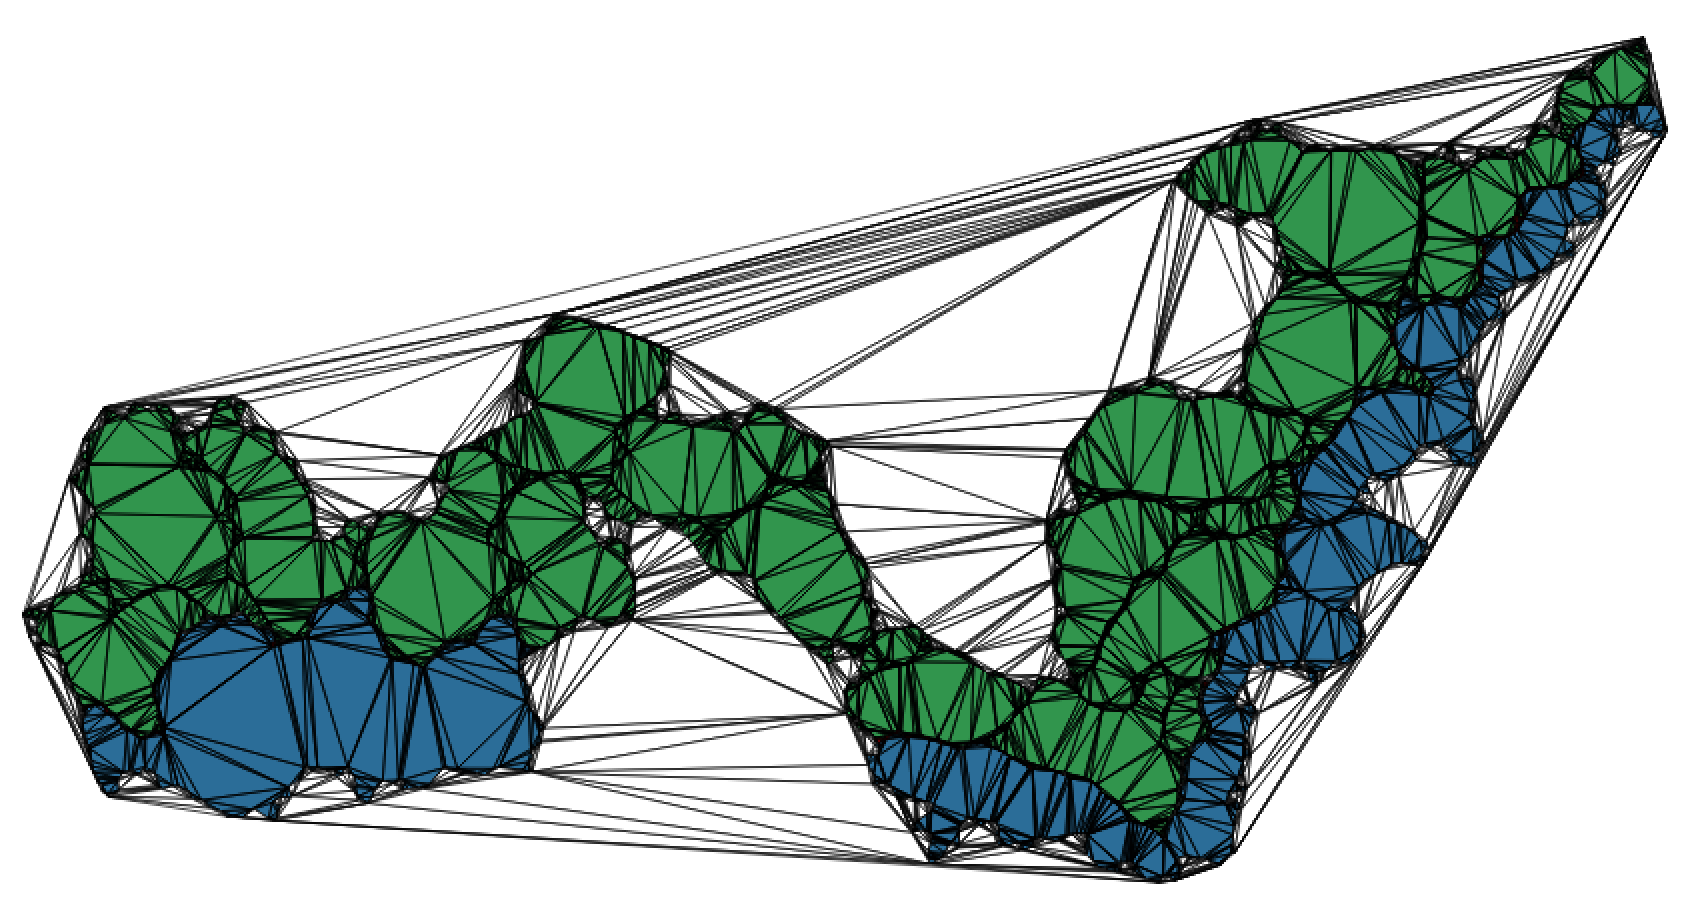
\includegraphics[width=0.8\linewidth]{figs/sometriangles.png}
  \caption{One nice figure}%
\label{fig:sometriangles}
\end{figure}
Notice that all figures in your thesis should be referenced to in the main text.
The same applies to tables and algorithms.

It is recommended \emph{not} to force-place your figures (\eg\ with commands such as: \texttt{\textbackslash{}newpage} or by forcing a figure to be at the top of a page).
\LaTeX\ usually places the figures automatically rather well.
Only if at the end of your thesis you have small problem then can you solve them.

As shown in \autoref{fig:sidebyside},
\begin{figure}
  \centering
  \begin{subfigure}[b]{0.3\linewidth}
    \centering
    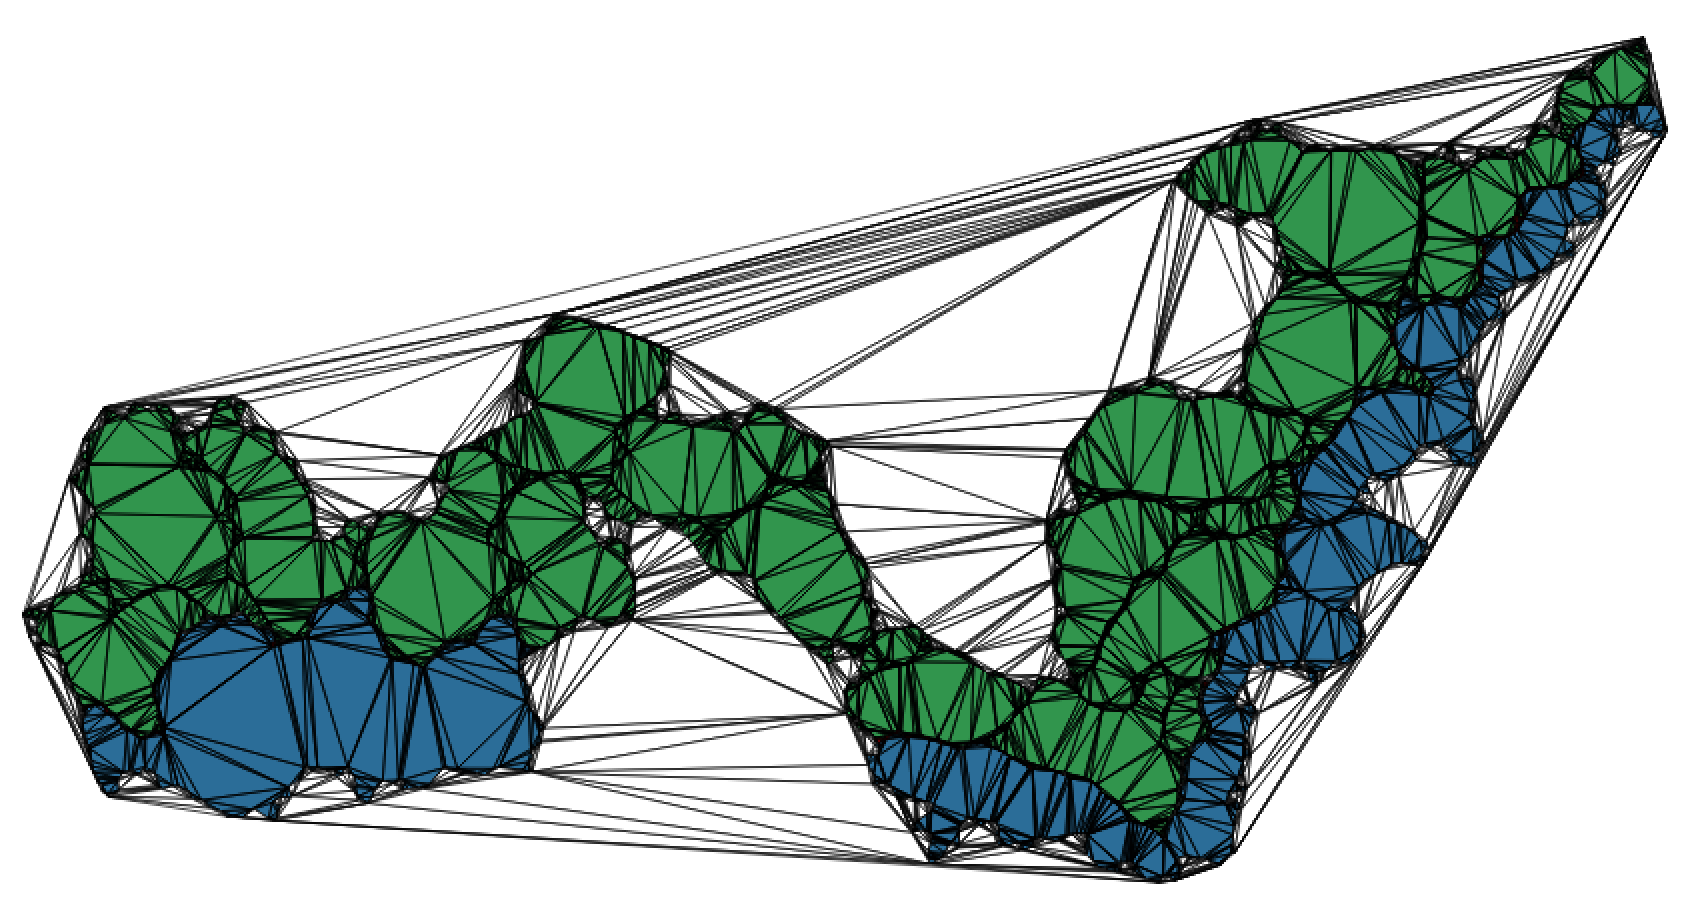
\includegraphics[angle=90,width=\linewidth]{figs/sometriangles.png}
    \caption{}\label{fig:sidebyside:1}
  \end{subfigure}%
  \qquad %-- that adds some space between th 2 figures
  \begin{subfigure}[b]{0.6\linewidth}
    \centering
    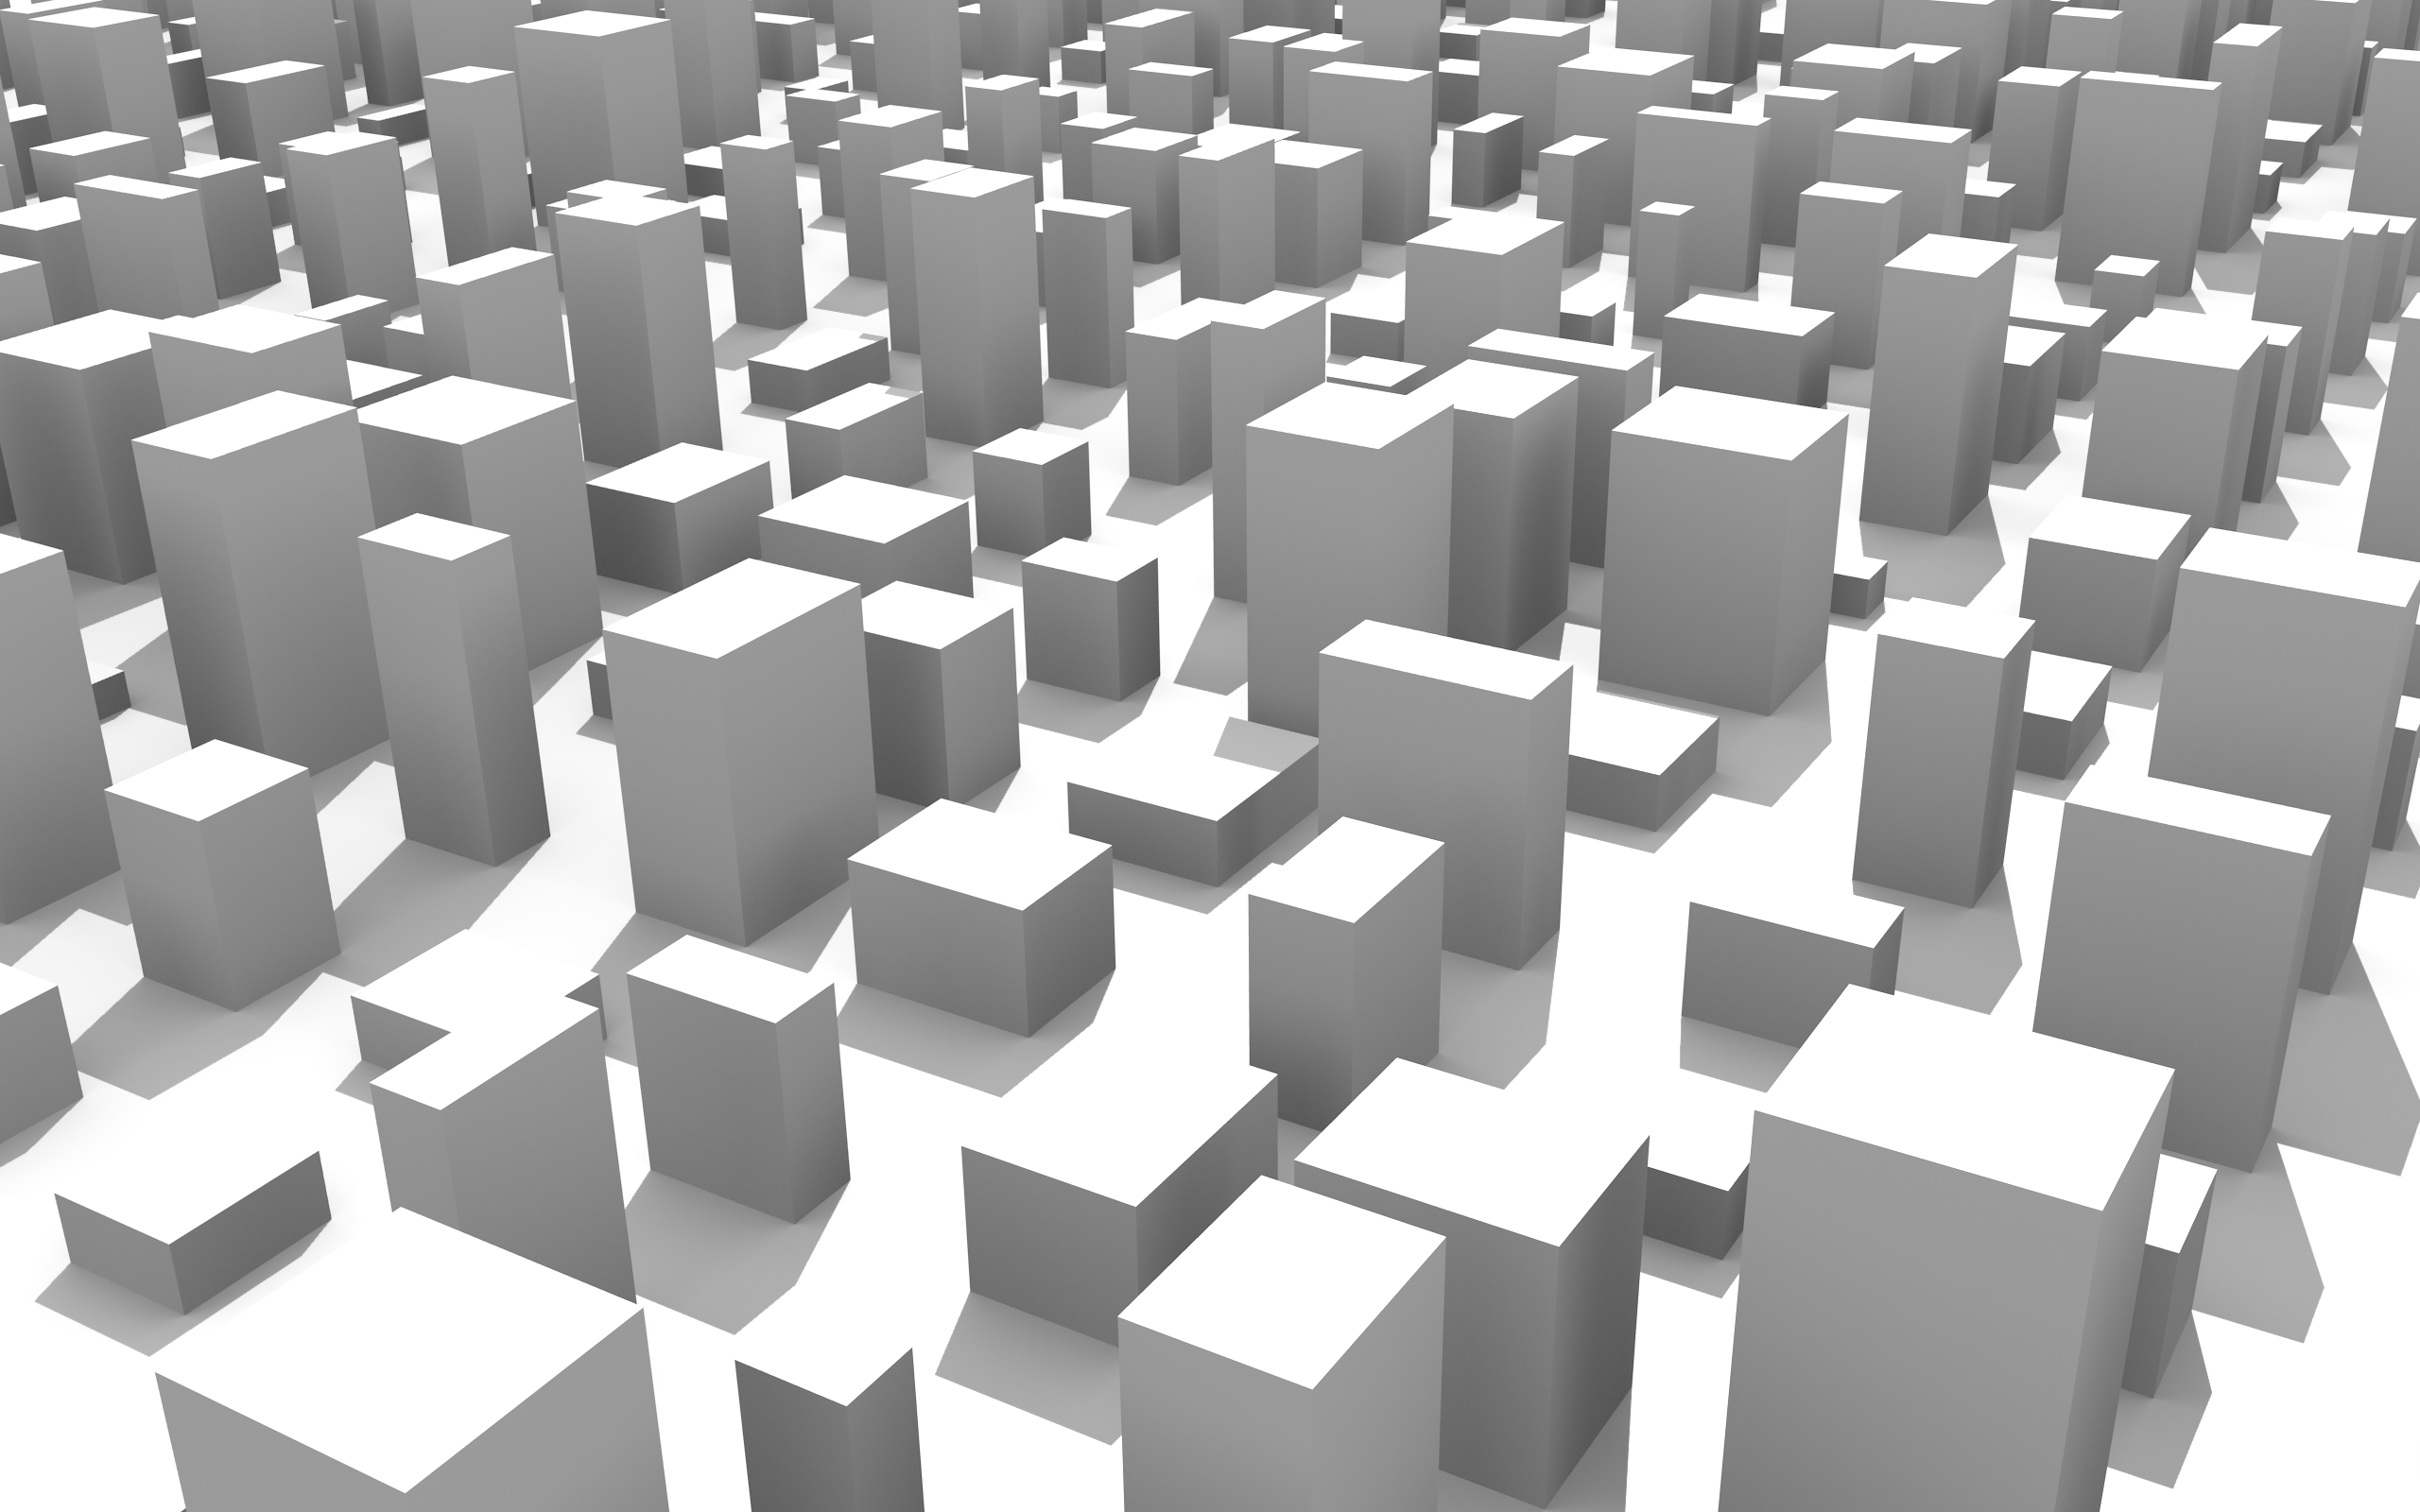
\includegraphics[width=\linewidth]{figs/lod1.png}
    \caption{}\label{fig:sidebyside:2}
  \end{subfigure}%
  \caption[Shortened title for the list of figures]{Two figures side-by-side. (a) A triangulation of 2 polygons. (b) Something not related at all.}%
\label{fig:sidebyside}
\end{figure}
it is possible to have two figures (or more) side by side.
You can also refer to a subfigure: see \autoref{fig:sidebyside:2}.


\subsection[Shorter section name for the TOC]{Figures in PDF are possible and even encouraged!}%
\label{sec:pdf}

If you use Adobe Illustrator or \href{http://ipe7.sourceforge.net}{Ipe} you can make your figures vectorial and save them in PDF\@.

You include a PDF the same way as you do for a PNG, see \autoref{fig:pdffig},
\begin{figure}
  \centering
  \begin{subfigure}[b]{0.28\linewidth}
    \centering
    
\includegraphics[page=1,width=\linewidth]{figs/tricat.pdf}
    \caption{2 polygons}\label{fig:pdffig:1}
  \end{subfigure}%
  \qquad %-- that adds some space between th 2 figures
  \begin{subfigure}[b]{0.28\linewidth}
    \centering
    
\includegraphics[page=2,width=\linewidth]{figs/tricat.pdf}
    \caption{CDT }\label{fig:pdffig:2}
  \end{subfigure}%
  \qquad %-- that adds some space between th 2 figures
  \begin{subfigure}[b]{0.28\linewidth}
    \centering
    
\includegraphics[page=3,width=\linewidth]{figs/tricat.pdf}
    \caption{with colours}\label{fig:pdffig:3}
  \end{subfigure}%
  \caption{Three PDF figures.}%
\label{fig:pdffig}
\end{figure}


%%%
%
\section{How to add references?}

References are best handled using Bib\TeX.
See the \texttt{myreferences.bib} file.
A good cross-platform reference manager is \href{http://jabref.sourceforge.net/}{JabRef}.

% \citet{Descartes37} wrote this and that~\citep{Voronoi08,Delaunay34}.
% Instead of citing the whole paper~\citep{Delaunay34}, it is also possible to cite only the authors (\eg\ \citeauthor{Delaunay34}).

%%%
%
\section{Footnotes}

Footnotes are a good way to write text that is not essential for the understanding of the text\footnote{but please do not overuse them}.

%%%
%
\section{Equations}

Equations and variables can be put inline in the text, but also numbered.

Let $S$ be a set of points in $\mathbb{R}^d$.
The Voronoi cell of a point $p \in S$, defined $\mathcal{V}_{p}$, is the set of points $x \in \mathbb{R}^d$ that are closer to $p$ than to any other point in $S$; that is:
\begin{equation}
\mathcal{V}_p = \{x \in \mathbb{R}^{d} \ | \ \|x-p\| \, \leq \, \|x-q\|, \ \forall \, q \in S \}.
\end{equation}
The union of the Voronoi cells of all generating points $p \in S$ form the Voronoi diagram of $S$, defined VD($S$).



%%%
%
\section{Tables}

The package \texttt{booktabs} permits you to make nicer tables than the basic ones in \LaTeX.
See for instance \autoref{tab:example}.
\begin{table}
  \centering
  \begin{tabular}{@{}lrrcrrc@{}} \toprule
    & \multicolumn{2}{c}{3D model} && \multicolumn{2}{c}{input} \\
    \cmidrule{2-3}  \cmidrule{5-6}
    & solids & faces && vertices & constraints  \\
    \toprule
    \textbf{campus}  & 370   & 4~298  && 5~970  & 3~976   \\
    \textbf{kvz}     & 637   & 6~549  && 8~951  & 13~571  \\
    \textbf{engelen} & 1~629 & 15~870 && 23~732 & 15~868 \\
    \bottomrule
   \end{tabular}
  \caption{Details concerning the datasets used for the experiments.}%
\label{tab:example}
\end{table}


%%%
%
\section{Plots}

The best way is to use \href{http://matplotlib.org}{matplotlib}, or its more beautiful version (\href{http://stanford.edu/~mwaskom/software/seaborn/index.html}{seaborn}).
With these, you can use Python to generate nice PDF plots, such as that in Figure~\ref{fig:myplot}.
\begin{figure}
  \centering
  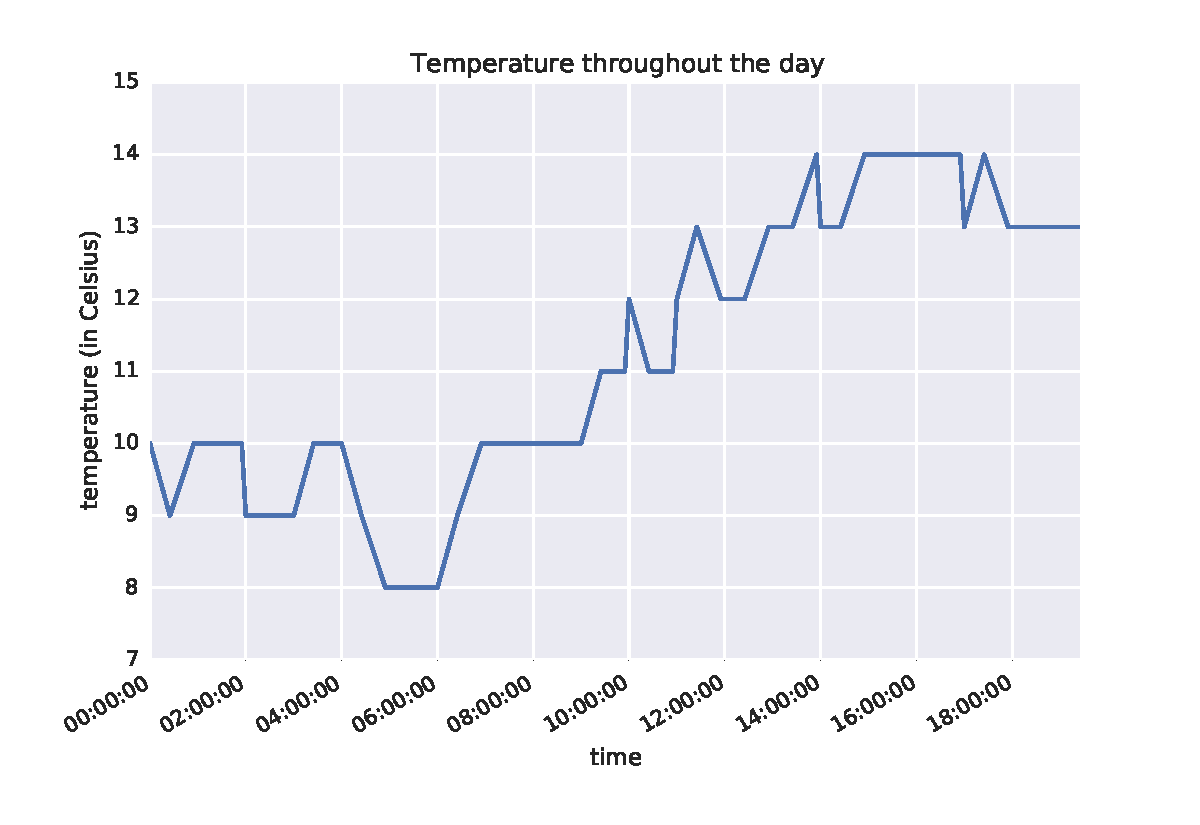
\includegraphics[width=0.95\linewidth]{plots/myplot.pdf}
  \caption{A super plot}%
\label{fig:myplot}
\end{figure}

In the folder \texttt{./plots/}, there is an example of a CSV file of the temperature of Delft, taken somewhere.
From this CSV, the plot is generated with the script \texttt{createplot.py}.


%%%
%
\section{Pseudo-code}%
\label{sec:code}

Please avoid putting code (Python, C++, Fortran) in your thesis.
Small excerpt are probably fine (for some cases), but do not put all the code in an appendix.
Instead, put your code somewhere online (\eg\ GitHub) and put \emph{pseudo-code} in your thesis.
The package \texttt{algorithm2e} is pretty handy, see for instance the \autoref{alg:walk}.
All your algorithms will be automatically added to the list of algorithms at the begining of the thesis.
\begin{algorithm}
  \KwIn{A Delaunay tetrahedralization $\mathcal{T}$, a starting tetrahedron $\tau$, and a query point $p$}
  \KwOut{$\tau_r$: the tetrahedron in $\mathcal{T}$ containing $p$}
  \BlankLine
  \While{$\tau_r$ not found}
  {
    \For{$i \leftarrow 0$ \KwTo 3}
    {
      $\sigma_i \leftarrow$ get face opposite vertex $i$ in $\tau$\;
      \If{Orient($\sigma_i, p$) $< 0$\nllabel{l:walk}}
      {
        $\tau \leftarrow$ get neighbouring tetrahedron of $\tau$ incident to $\sigma_i$\;
        break\;
      }
    }
    \If{$i=3$}
    {
      \tcp{all the faces of $\tau$ have been tested}
      \Return{$\tau_r$ = $\tau$}
    }
  }
  \caption[W\textsc{alk}]{W\textsc{alk} ($\mathcal{T}$, $\tau$, $p$)}%
\label{alg:walk}
\end{algorithm}
Observe that you can put labels on certain lines (with \texttt{\nllabel{}}) and then reference to them: on line~\ref{l:walk} of the \autoref{alg:walk} this is happening.

If you want to put some code (or XML for instance), use the package \texttt{listings}, \eg\ you can wrap it in a Figure so that it does not span over multiple pages.
\begin{figure}
\begin{footnotesize}
\begin{lstlisting}
<gml:Solid>
  <gml:exterior>
    <gml:CompositeSurface>
      <gml:surfaceMember>
        <gml:Polygon>
          <gml:exterior>
            <gml:LinearRing>
              <gml:pos>0.000000 0.000000 1.000000</gml:pos>
              <gml:pos>1.000000 0.000000 1.000000</gml:pos>
              <gml:pos>1.000000 1.000000 1.000000</gml:pos>
              <gml:pos>0.000000 1.000000 1.000000</gml:pos>
              <gml:pos>0.000000 0.000000 1.000000</gml:pos>
            </gml:LinearRing>
          </gml:exterior>
          <gml:interior>
          ...
      </gml:surfaceMember>
    </gml:CompositeSurface>
  </gml:interior>
</gml:Solid>
\end{lstlisting}
\end{footnotesize}
\caption{Some GML for a \texttt{gml:Solid}.}%
\label{fig:codegml}
\end{figure}

%%%
%
\section{Acronyms}%
\label{sec:acronyms}

If you want to have a list of acronyms you use in your thesis, use the \texttt{acronym} package.
The first time you speak about \ac{gis}, it will be spelled out.
Further use, \ac{gis}, you'll get the acronym plus a hyperlink to the list in the preambule of the thesis.

Add yours to \texttt{front/acronyms.tex}.
Notice that only these used are printed, \eg\ \ac{dt} and \ac{tin}.


%%%
%
\section{TODO notes}%
\label{sec:todo}

At P4 or for earlier drafts, it might be good to let the readers know that some part need more work.
Or that a figure will be added.

The package \href{http://tug.ctan.org/macros/latex/contrib/todonotes/todonotes.pdf}{todonotes} is perfect for this.
\todo{adding holders for figures is also possible}

A summary of all TODOs in the thesis can even be generated.

%%%
%
\section{Miscellaneous}%
\label{sec:misc}

In the file \texttt{mysettings.tex}, there are some handy shortcuts.

This is the way to properly write these abbreviations, \ie\ so that the spacing is correct.
And this is how you use an example, \eg\ like this.

You should use one \texttt{-} for an hyphen between words (`multi-dimensional'), two \texttt{--} for a range between numbers (`1990--1995'), and three \texttt{---} for a punctuation in a sentence (`I like---unlike my father---to build multi-dimensional models').
